% Online Appendix to Section 11 (sec:robustness). Numbers: paper/results/robustness.json
% (scripts/paper/fig_robustness.R; final rerun of 2026-10-12, the October 2026 NIPO component, the
% vertical-complementarity study of 2026-10-12 and the CM-FDI integration study on the inputs of
% 2026-10-11). Tables: paper/tables/robustness_*.tex (generated).
\section{Robustness and validation: further detail}\label{oa:robustness}

\paragraph{Reproduction.} The weighting experiments use a re-implementation of the available-case
mean of equation~\eqref{eq:pillar} on the stored category scores, which reproduces the stored
indices at the configured weights to within $10^{-15}$; the curvature, imputation and data-choice
experiments rebuild both pillars from the theme tables with the pipeline's builders and
configuration; the Strategic Index and the Policy index are rebuilt with the pipeline's own
functions. Each reproduces the stored values exactly at the baseline settings.
Table~\ref{tab:robustness_summary} collects the within-pair correlations of the pillars.

% Generated by scripts/paper/fig_robustness.R; do not edit by hand.
\begin{table}[tbp]
  \centering
  \begin{threeparttable}
  \caption{Robustness of within-pair country rankings: Spearman correlations with the baseline}
  \label{tab:robustness_summary}
  \small
  \begin{tabular}{lcccccc}
    \toprule
     & \multicolumn{3}{c}{Energy Security ($\ES$)} & \multicolumn{3}{c}{Economic Opportunity ($\EO$)} \\
    \cmidrule(lr){2-4}\cmidrule(lr){5-7}
    Variant & Pooled & Median & Minimum & Pooled & Median & Minimum \\
    \midrule
    \multicolumn{7}{l}{\emph{Category weights}}\\
    \quad Dirichlet draws & 0.99 & 1.00 & 0.98 & 0.98 & 0.99 & 0.97 \\
    \quad Equal weights & 0.97 & 1.00 & 0.98 & 0.98 & 1.00 & 1.00 \\
    \multicolumn{7}{l}{\emph{S-curve curvature} (baseline $\gamma=0.5$)}\\
    \quad $\gamma=0.25$ & 0.98 & 1.00 & 0.97 & 0.98 & 0.99 & 0.98 \\
    \quad $\gamma=1$ (percent rank) & 0.98 & 0.99 & 0.90 & 0.98 & 0.99 & 0.97 \\
    \quad $\gamma=2$ & 0.93 & 0.96 & 0.74 & 0.94 & 0.97 & 0.90 \\
    \multicolumn{7}{l}{\emph{Global-average imputation rules}}\\
    \quad Removed (available case) & 0.99 & 1.00 & 0.62 & 0.85 & 0.97 & 0.29 \\
    \quad Replaced by zero & 0.87 & 0.98 & 0.58 & 0.62 & 0.77 & 0.42 \\
    \multicolumn{7}{l}{\emph{Vintage}}\\
    \quad 2020 against 2025 & 0.97 & 0.99 & 0.68 & 0.89 & 0.87 & 0.49 \\
    \quad 2025 vintage against headline & 0.99 & 1.00 & 0.87 & 0.99 & 1.00 & 0.79 \\
    \bottomrule
  \end{tabular}
  \begin{tablenotes}[flushleft]\footnotesize
    \item \emph{Notes:} Spearman rank correlations between the baseline pillar and each variant, over the baseline's rankable cells (sovereign economies with at most half of the index weight imputed). ``Pooled'' is computed over all rankable cells of the eleven headline technologies; ``Median'' and ``Minimum'' are taken across technology--stage pairs of the correlation computed within each pair. For the Dirichlet draws the pooled entry is the median over 1{,}000 draws and the within-pair entries summarise, across pairs, each pair's median over the draws. The vintage rows compare the 2020 and 2025 builds of \texttt{scripts/40\_build\_index\_vintages.R}, in which only the time-varying sources differ (4{,}139 $\ES$ and 4{,}301 $\EO$ rankable cells observed in both vintages), and the 2025 build with the headline index. Sample: 30 $\ES$ pairs (4{,}163 rankable cells) and 33 $\EO$ pairs (4{,}301 rankable cells). Entries are rounded to two decimals. Source: \texttt{scripts/paper/fig\_robustness.R}; \texttt{paper/results/robustness.json}.
  \end{tablenotes}
  \end{threeparttable}
\end{table}


\paragraph{Vintages.} A separate build re-derives both pillars as of 2020 and 2025 by slicing the
time-varying sources (the EI Statistical Review, the Atlas of Economic Complexity, GCIM investment,
and the IMF and ILO price, rate and earnings series) to each year, holding the other themes
(resource potential, reserves, the IEA critical-mineral and clean-technology tables, the mineral
production sheets, BNEF demand, levelised costs, overcapacity and technology readiness) identical,
and measuring Trade on the Atlas basis. Categories carrying 52 per cent of the nominal $\ES$ weight
and 70 per cent of the $\EO$ weight are time-varying by classification, those whose scores differ in
at least one per cent of their cells 40 and 50 per cent, and, after renormalisation over observed
categories, 34 per cent of the average $\ES$ cell's weight and 36 per cent of the average $\EO$
cell's re-derive. In $\ES$ (Figure~\ref{fig:robustness_vintage}) the mean absolute change is 0.015,
31 per cent of cells do not change, and the mean percentile shift is 3.8 points; 77 per cent of the
squared Upstream changes is a common shift of whole pairs from the Energy Prices category, which is
constant within a pair. In $\EO$ the mean absolute change is 0.030, no cell is unchanged and the mean
percentile shift is 10.8 points, because Cost Competitiveness re-derives in every pair from annual
earnings, lending-rate and producer-price series. Oil Downstream has the lowest correlation in both
pillars (0.68 and 0.49). The largest single moves occur where a pair rests on one flow variable: in
Electric Vehicles Downstream $\ES$, built from annual GCIM flows alone, Viet Nam moves from 94th of
101 to 3rd. The 2025 vintage coincides with the headline except in Trade (median within-pair
correlation 1.00 in both pillars; minima 0.87 in $\ES$ Nuclear Midstream and 0.79 in $\EO$ Nuclear
Upstream, whose baskets the final revision changed). Because only about a third of the weight
re-derives, the comparison likely understates instability over time; the vintage years are nominal
for two sources (Atlas 2023 in the 2025 vintage, IMF producer prices 2021 in the 2020 vintage).

\begin{figure}[tbp]
  \centering
  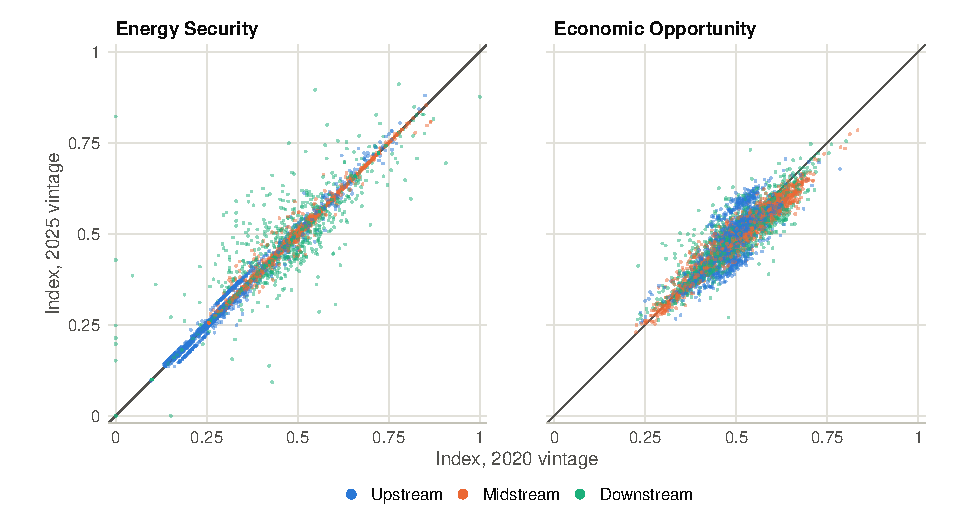
\includegraphics[width=\textwidth]{robustness_vintage}
  \caption{The 2020 and 2025 vintages of the pillars. Each point is a rankable country cell of the
  eleven headline technologies observed in both vintages (4{,}139 in $\ES$, 4{,}301 in $\EO$),
  coloured by stage; the line is the 45-degree line. Both vintages are built by
  \texttt{scripts/40\_build\_index\_vintages.R} with the headline builders and configuration; only
  the time-varying sources are sliced to the vintage year, and Trade is measured on the Atlas basis.
  Source: \texttt{data/processed/vintages}; \texttt{scripts/paper/fig\_robustness.R}.}
  \label{fig:robustness_vintage}
\end{figure}

\paragraph{Category weights.} The weight vectors are drawn as $w\sim\mathrm{Dir}(c\,\bar w)$ around
the configured shares $\bar w$, so that $E[w_k]=\bar w_k$ and the coefficient of variation of $w_k$
is $\sqrt{(1-\bar w_k)/[\bar w_k(c+1)]}$; $c=99$ for the ten categories of a pillar gives 0.3 for a
category of average weight \citep{decancq2013weights}. In seven $\ES$ pairs and three $\EO$ pairs a
single category varies, and there the ranking does not depend on the weights at all; on average 3
per cent of the observed weight of an $\ES$ pair and 25 per cent of an $\EO$ pair sits on categories
constant within it. Restricted to pairs with two or more varying categories (23 in $\ES$, 30 in
$\EO$), the median correlation over pair--draws is 0.996 and 0.987, but the minimum falls to 0.77
and 0.30. For each coalition member and pair, the 5th to 95th percentile band of its percentile
position over the draws has a median width of 2.8 points in $\ES$ (1{,}606 member cells) and 9.6 in
$\EO$ (1{,}718), with a 90th percentile of 18 and 31 points. Wide bands arise among large blocks of
tied scores: in $\ES$ Batteries Downstream South Korea ranks 69th of 186 at the configured weights
with a band from 15th to 186th; in $\EO$ the widest bands are Upstream, such as Brazil in Nuclear
Upstream (163rd of 175, band 21st to 174th). Figure~\ref{fig:robustness_ranks} shows one pair.

\begin{figure}[tbp]
  \centering
  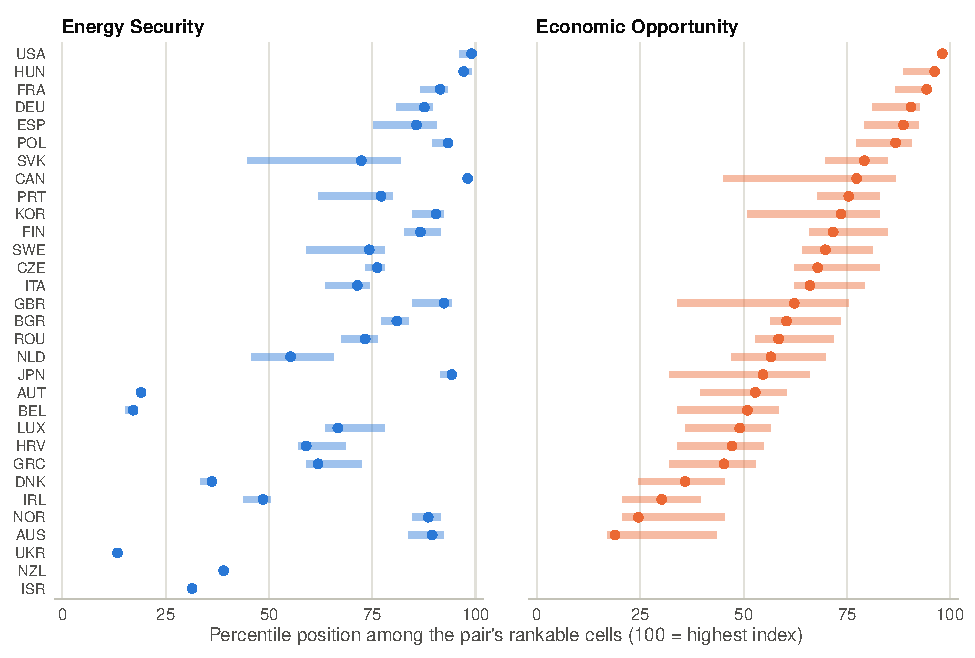
\includegraphics[width=\textwidth]{robustness_ranks}
  \caption{Rank uncertainty of the core members under perturbed category weights, Batteries
  Midstream. For each core member with a rankable cell (31 in $\ES$, 28 in $\EO$) the dot is its
  percentile position at the configured weights and the bar spans the 5th to 95th percentiles over
  1{,}000 Dirichlet draws (coefficient of variation 0.3 for a category of average weight). Source:
  category scores in \texttt{index\_outputs.rds}; \texttt{scripts/paper/fig\_robustness.R}.}
  \label{fig:robustness_ranks}
\end{figure}

\paragraph{Curvature.} Because $\operatorname{logit}\Scurve(r)=\gamma\operatorname{logit}r$, a
component at curvature $\gamma'$ follows from the stored value as
$\phi_{\gamma'}(r)=\operatorname{logistic}\big((\gamma'/0.5)\operatorname{logit}\phi_{0.5}(r)\big)$,
which also maps anchored zeros to zero. The map is exact for a component that is a single S-curve of
a rank; 46 of the 57 components that enter a scored category pass this test, carrying 84 per cent
of the average $\ES$ cell's weight and 63 per cent of the $\EO$ cell's. For the others (the input-
and levelised-cost terms, readiness, overcapacity, the production surplus of Energy Imports, the
mineral-supply and production shares of Foreign Dependency, the minerals-trade terms and the
geothermal and wind potential indices) it re-curves a mean and is an approximation. Levels move more
than ranks: the mean absolute change of $\ES$ is 0.03, 0.04 and 0.08 at $\gamma'=0.25$, 1 and 2.

\paragraph{Imputation.} Nine $\ES$ themes and twelve $\EO$ themes fill uncovered countries with the
observed mean of their component group (equation~\eqref{eq:impute}). Such components carry on average
7 per cent of an $\ES$ cell's weight, mainly in Energy Access and Foreign Dependency, and 25 per cent
of an $\EO$ cell's, two thirds of it in Technology Demand and most of the rest in Production and Cost
Competitiveness. The lowest within-pair correlations are Nuclear Upstream (0.62) without imputation
and Coal Downstream (0.58) with zeros in $\ES$, and Coal Midstream (0.29) without imputation in
$\EO$. Zero-filling places every uncovered economy at or below every covered one on the component;
removing the rule scores it on fewer measurements than its neighbours; the global average compresses
the differences the component would make. None is neutral.

\paragraph{Rankability.} Table~\ref{tab:robustness_rankability} varies $\tau$. Because the rule
filters cells without changing values, it changes the sample, not the order of cells rankable under
both thresholds. At $\tau=0.3$ the rankable cells are 56 per cent of the sovereign scored cells in
$\ES$ and 31 per cent in $\EO$ (74 and 67 per cent at the headline), at $\tau=0.7$ 95 and 93 per
cent. The median within-pair correlation of $\EO$ with its zero-filled variant is 0.94 at $\tau=0.3$,
0.77 at the headline and 0.68 at $\tau=0.7$. The top ten of 27 of the 30 $\ES$ pairs are identical at
$\tau=0.3$ but only 15 of the 33 $\EO$ top-ten lists. At $\tau=0.3$, 48 of the 57 members keep a pick
and 29 of them the baseline one; at $\tau=0.7$, 42 of 57 keep the baseline pick. At $\tau=0.3$ the
world view of the PSI ranks 102 partners and the core view 159.

% Generated by scripts/paper/fig_robustness.R; do not edit by hand.
\begin{table}[tbp]
  \centering
  \begin{threeparttable}
  \caption{The rankability threshold: cells ranked, robustness of their rankings, and the Strategic Index}
  \label{tab:robustness_rankability}
  \small
  \begin{tabular}{lcccccccccc}
    \toprule
    & \multicolumn{3}{c}{$\ES$} & \multicolumn{3}{c}{$\EO$} & \multicolumn{3}{c}{Strategic Index} & PSI \\
    \cmidrule(lr){2-4}\cmidrule(lr){5-7}\cmidrule(lr){8-10}\cmidrule(lr){11-11}
    $\tau$ & Cells & $\rho_{\text{none}}$ & $\rho_{\text{zero}}$ & Cells & $\rho_{\text{none}}$ & $\rho_{\text{zero}}$ & Cells & Countries & Picks & Ranked \\
    \midrule
    0.3 & 3{,}147 & 1.00 & 1.00 & 1{,}967 & 0.99 & 0.94 & 1{,}577 & 107 & 29/48 & 159/102 \\
    0.5$^{\ast}$ & 4{,}163 & 1.00 & 0.98 & 4{,}301 & 0.97 & 0.77 & 3{,}154 & 174 & 57/57 & 192/188 \\
    0.7 & 5{,}350 & 0.99 & 0.98 & 5{,}974 & 0.86 & 0.68 & 5{,}156 & 194 & 42/57 & 194/194 \\
    \bottomrule
  \end{tabular}
  \begin{tablenotes}[flushleft]\footnotesize
    \item \emph{Notes:} A cell is rankable when the economy is sovereign and at most a share $\tau$ of its index weight rests on imputed components ($^{\ast}$ the headline, \texttt{config/rankability.yml}). Cells: rankable headline cells (of 6{,}232 scored $\ES$ and 7{,}131 scored $\EO$ cells). $\rho_{\text{none}}$ and $\rho_{\text{zero}}$: median across technology--stage pairs of the within-pair Spearman correlation, over the cells rankable at $\tau$, between the baseline pillar and the pillar rebuilt with every global-average rule removed (available case) or replaced by zero. Strategic Index: cells and countries in the sample when the pillars' rankable flags are taken at $\tau$ (the Policy index is unchanged), and the number of coalition members whose allied pick is the baseline one, over the members with a pick at $\tau$. PSI: partners ranked in the core-coalition (headline) and world views. Within a technology--stage pair the order of two cells rankable under two thresholds is the same, because the rule filters cells and does not change values. Source: \texttt{scripts/paper/fig\_robustness.R} (\texttt{rankability} in \texttt{paper/results/robustness.json}).
  \end{tablenotes}
  \end{threeparttable}
\end{table}


\paragraph{Leave one category out and effective importance.} Figure~\ref{fig:robustness_loo} drops
one category at a time. In $\ES$ the ranking depends most on Consumption (median within-pair
correlation 0.74 over eight pairs) and Minerals Trade (0.79 over six); Trade has the widest range
(minimum 0.40 in Electric Grid Midstream, whose basket the completed trade file filled) and is the
only category of the four Midstream fossil and nuclear pairs. Production and Foreign Dependency,
which share the largest nominal $\ES$ weight, change almost nothing (0.995 and 0.998). In $\EO$,
Foreign Dependency (0.75), Cost Competitiveness (0.76) and Trade (0.79) carry most of the ranking,
while Technology Demand changes it little (0.99) and Technological Readiness and Energy Prices,
constant within pairs, not at all. A complementary, exact measure is the share of a pillar's
cross-country variance within a pair for which each category accounts. Because the pillar is the sum
of its category contributions $C_{kits}$ (equation~\eqref{eq:cat_decomp}),
\begin{equation}\label{eq:variance_share}
  S_{kts}=\frac{\operatorname{Cov}_i\bigl(C_{kits},\,\ES_{its}\bigr)}
               {\operatorname{Var}_i\bigl(\ES_{its}\bigr)},
  \qquad \sum_{k}S_{kts}=1,
\end{equation}
and likewise for $\EO$, a linear counterpart of the main effects of \citet{paruolo2013ratings}.
Table~\ref{tab:robustness_importance} compares nominal weights, mean effective weights and mean
variance shares. The share of weight that would have to move for nominal and variance shares to
coincide is 0.32 in $\ES$ and 0.37 in $\EO$. In $\ES$ the gap is mainly coverage: Trade, observed in
18 of the 30 pairs, has 9.5 per cent of the nominal weight but 24.9 per cent of the effective weight
and 21.5 per cent of the variance. In $\EO$ it arises within pairs: Technology Demand and
Technological Readiness hold 21.8 and 14.6 per cent of the effective weight but 3.6 and 0.0 per cent
of the variance, while Cost Competitiveness holds 21.9 and 32.8 per cent.

\begin{figure}[tbp]
  \centering
  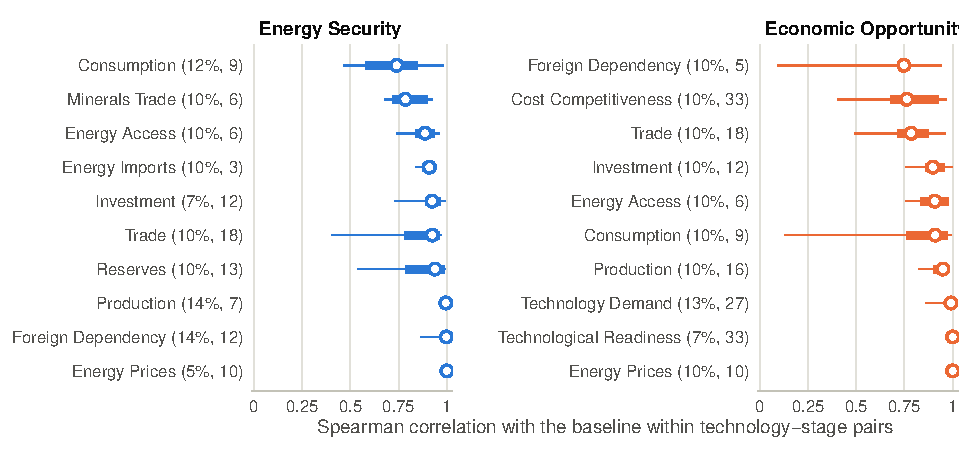
\includegraphics[width=\textwidth]{robustness_loo}
  \caption{Leave-one-category-out sensitivity of within-pair rankings: Spearman correlation between
  the baseline and the pillar without the category (remaining categories renormalised), over the
  pairs in which the category is observed and the baseline's rankable cells; open circle, median;
  thick bar, interquartile range; thin line, range. Labels give the nominal weight share and the
  number of pairs observed. Pairs in which the dropped category is the only varying one are omitted.
  Source: \texttt{index\_outputs.rds}; \texttt{scripts/paper/fig\_robustness.R}.}
  \label{fig:robustness_loo}
\end{figure}

% Generated by scripts/paper/fig_robustness.R; do not edit by hand.
\begin{table}[tbp]
  \centering
  \begin{threeparttable}
  \caption{Nominal weight, effective weight and variance share of each category within technology--stage pairs}
  \label{tab:robustness_importance}
  \small
  \begin{tabular}{lrrrrr}
    \toprule
    & Nominal & Effective & Variance & & Leave-one- \\
    Category & share (\%) & weight (\%) & share (\%) & Pairs & out $\rho$ \\
    \midrule
    \multicolumn{6}{l}{\emph{Panel A. Energy Security ($\ES$), 30 pairs}}\\
    \quad Trade & 9.5 & 24.9 & 21.5 & 18 & 0.93 \\
    \quad Investment & 7.1 & 11.3 & 18.1 & 12 & 0.92 \\
    \quad Reserves & 9.5 & 9.5 & 17.4 & 13 & 0.94 \\
    \quad Consumption & 11.9 & 15.8 & 13.2 & 9 & 0.74 \\
    \quad Foreign Dependency & 14.3 & 16.1 & 10.1 & 12 & 1.00 \\
    \quad Production & 14.3 & 5.8 & 10.0 & 7 & 0.99 \\
    \quad Energy Access & 9.5 & 7.2 & 5.0 & 6 & 0.89 \\
    \quad Energy Imports & 9.5 & 2.9 & 2.8 & 3 & 0.91 \\
    \quad Minerals Trade & 9.5 & 3.1 & 1.8 & 6 & 0.79 \\
    \quad Energy Prices & 4.8 & 3.4 & 0.0 & 10 & 1.00 \\
    \addlinespace
    \multicolumn{6}{l}{\emph{Panel B. Economic Opportunity ($\EO$), 33 pairs}}\\
    \quad Cost Competitiveness & 10.0 & 21.9 & 32.8 & 33 & 0.76 \\
    \quad Trade & 10.0 & 11.0 & 17.5 & 18 & 0.79 \\
    \quad Investment & 10.0 & 6.6 & 14.4 & 12 & 0.90 \\
    \quad Production & 10.0 & 8.1 & 12.5 & 16 & 0.95 \\
    \quad Consumption & 10.0 & 5.0 & 7.9 & 9 & 0.91 \\
    \quad Foreign Dependency & 10.0 & 2.9 & 7.4 & 5 & 0.75 \\
    \quad Energy Access & 10.0 & 2.8 & 3.8 & 6 & 0.91 \\
    \quad Technology Demand & 13.3 & 21.8 & 3.6 & 27 & 0.99 \\
    \quad Energy Prices & 10.0 & 5.3 & 0.0 & 10 & 1.00 \\
    \quad Technological Readiness & 6.7 & 14.6 & 0.0 & 33 & 1.00 \\
    \bottomrule
  \end{tabular}
  \begin{tablenotes}[flushleft]\footnotesize
    \item \emph{Notes:} Nominal share: $w_k/\sum_{k'}w_{k'}$ from \texttt{config/weights.yml}. Effective weight: mean over the rankable headline pairs of the weight $w_k/\sum_{l\ \mathrm{observed}}w_l$ a category receives after renormalisation over the observed categories; zero where the category is not observed. Variance share: mean over the same pairs of $S_{kts}$ (equation~\eqref{eq:variance_share}), the covariance of the category's contribution with the pillar across the rankable cells of the pair divided by the pillar's variance; zero where the category is not observed. Each of the three columns sums to 100 within a panel up to rounding. Pairs: number of pairs in which the category is observed. Leave-one-out $\rho$: median, over the pairs in which the category is observed and the reduced pillar still ranks countries, of the within-pair Spearman correlation between the baseline pillar and the pillar without the category (Figure~\ref{fig:robustness_loo}). Rows are ordered by the variance share. Sample: rankable cells of the eleven headline technologies. Source: category scores in \texttt{index\_outputs.rds}; \texttt{scripts/paper/fig\_robustness.R} (\texttt{weights.<pillar>.variance\_importance} in \texttt{paper/results/robustness.json}).
  \end{tablenotes}
  \end{threeparttable}
\end{table}


\paragraph{Strategic Index weights and policy variants.} The Dirichlet draws of the five weights of
equation~\eqref{eq:si} use concentration 43.4, giving coefficients of variation of 0.30 for the
policy weight, 0.23 for the two pillar weights and 0.45 for the two priors. Indonesia keeps its pick
in 15 per cent of the draws, its two leading sectors differing by 0.0007. Under security in place of
need, 28 members pick Nuclear Midstream and 10 Gas Midstream; without the priors, ten picks move to
Oil Midstream, the sector the technology prior penalises most; without the policy term, 20 members
pick Nuclear Upstream instead of 8. Requiring both Policy components leaves 1{,}666 Strategic Index
cells; dropping CAT for every country gives a median within-country Strategic Index correlation of
1.00 (interquartile range 0.91 to 1.00, minimum 0.30). The October 2026 NIPO component (GTA NIPO as of
5 October 2026, debiased strength; 1{,}070 rows), added with weights 4, 3 and 2 on NIPO, IEA PAMS and
CAT and IEA PAMS still required, is observed in Upstream and Midstream cells only, in 841 Strategic
Index cells (27 per cent); for its jurisdictions the within-country Spearman correlation between the
policy ranks with and without it has a median of 0.88 (range 0.00 to 1.00), the pooled Strategic
Index correlation is 0.97, and 27 of the 50 members with a NIPO score keep their pick.

\paragraph{Data choices of the final build.} Table~\ref{tab:robustness_data} and
Figure~\ref{fig:robustness_picks_data} report the data choices of the last revision (11--12 October
2026). The headline carries 807 EIA-sourced rows in the import-dependence theme and 656 in the
production theme; setting them to zero gives within-pair correlations of 0.97 to 0.98 in $\ES$ and
0.95 to 0.96 in $\EO$ in Oil, Gas and Coal Upstream. Removing Trade from the four Upstream cells with
new baskets gives median within-pair correlations of 0.94 in $\ES$ and 0.73 in $\EO$ (minimum 0.58,
Solar Upstream $\EO$) and returns the Strategic Index to 192 countries, because the newly imputed
Trade category had pushed small economies over the rankability threshold; three of the four changed
picks move to Nuclear Upstream. The superseded energy-trade file is not kept, but interim builds
record the picks: on 8 October, 45 of the 56 members then in the coalition had a pick, 17 Electric
Grid Midstream and 11 Batteries Midstream; on 10 October, 4 and 26 of 57. Without Trade, Electric
Grid Midstream picks rise to 10 and Batteries Midstream falls to 13; without Technological Readiness
32 of 57 picks survive (Electric Grid Midstream would take 27), without Technology Demand 41 and
without Foreign Dependency 44. The CM-FDI comparison is not re-run on the final outputs, because the
dyad tables exceed the memory budget of the replication; in the integration study, switching off the
Chinese-parent component or the CM-FDI investment ties alone gives core-PSI correlations of 0.9999.

\begin{figure}[tbp]
  \centering
  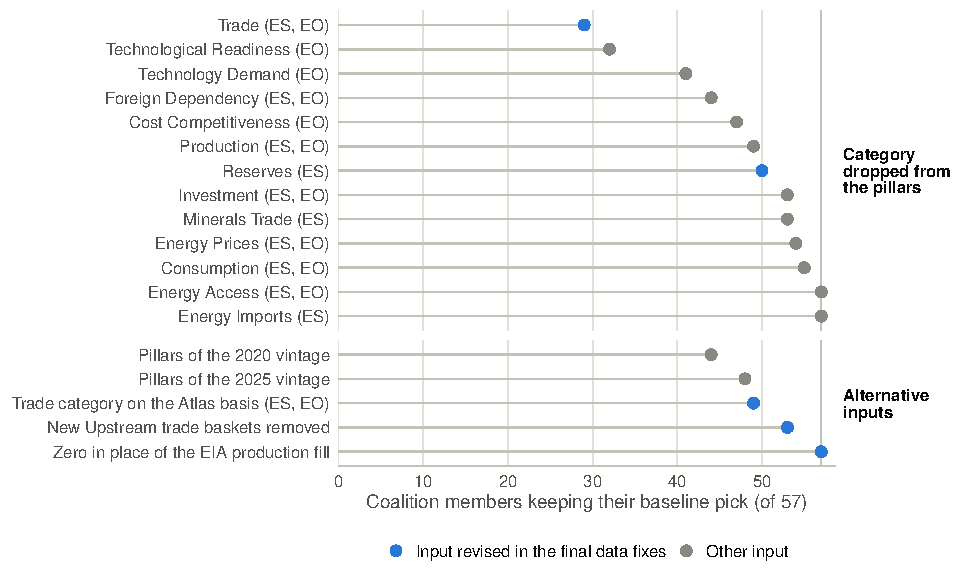
\includegraphics[width=\textwidth]{robustness_picks_data}
  \caption{Stability of the allied picks under the data inputs: number of members, of 57, whose pick
  is the baseline one when the Strategic Index takes pillars rebuilt under a variant. Upper panel:
  one category dropped (without Trade three members have no eligible rankable sector, so 29 of the
  54 with a pick keep it). Lower panel: pillars from the 2020 or 2025 vintage, Trade on the Atlas
  basis, Trade removed from the four Upstream cells whose baskets were added on 11 October 2026, and
  EIA-filled fossil production set to zero. Blue marks inputs revised in the final data fixes. The
  Policy index and the endowment screen are the headline ones. Source: \texttt{index\_outputs.rds},
  theme tables, vintages; \texttt{scripts/paper/fig\_robustness.R}.}
  \label{fig:robustness_picks_data}
\end{figure}

% Generated by scripts/paper/fig_robustness.R; do not edit by hand.
\begin{table}[tbp]
  \centering
  \begin{threeparttable}
  \caption{Data and policy choices of the final build: rankable cells, rankings and allied picks}
  \label{tab:robustness_data}
  \footnotesize
  \setlength{\tabcolsep}{4pt}
  \begin{tabular}{lccccccc}
    \toprule
    & \multicolumn{2}{c}{Rankable cells} & \multicolumn{2}{c}{Median $\rho$, touched pairs} & \multicolumn{3}{c}{Strategic Index} \\
    \cmidrule(lr){2-3}\cmidrule(lr){4-5}\cmidrule(lr){6-8}
    Variant & $\ES$ & $\EO$ & $\ES$ & $\EO$ & Cells & Countries & Same pick \\
    \midrule
    Baseline & 4{,}163 & 4{,}301 & -- & -- & 3{,}154 & 174 & 57/57 \\
    \multicolumn{8}{l}{\emph{Data}}\\
    \quad Zero in place of the EIA fill & 4{,}164 & 4{,}301 & 0.98 & 0.96 & 3{,}155 & 174 & 57/57 \\
    \quad New Upstream baskets removed & 4{,}161 & 4{,}307 & 0.94 & 0.73 & 3{,}144 & 192 & 53/57 \\
    \multicolumn{8}{l}{\emph{Policy index}}\\
    \quad Both components required & = & = & -- & -- & 1{,}666 & 65 & 46/46 \\
    \quad IEA PAMS alone & = & = & -- & -- & 3{,}154 & 174 & 45/57 \\
    \quad October 2026 NIPO added back & = & = & -- & -- & 3{,}154 & 174 & 34/57 \\
    \multicolumn{8}{l}{\emph{Allied pick rule}}\\
    \quad Endowment screen off & = & = & -- & -- & 3{,}154 & 174 & 16/57 \\
    \bottomrule
  \end{tabular}
  \begin{tablenotes}[flushleft]\footnotesize
    \item \emph{Notes:} Rankable cells: headline cells of sovereign economies with at most half of the index weight imputed, after the variant (= unchanged). Median $\rho$: median across the touched technology--stage pairs (Oil, Gas and Coal Upstream for the EIA fill; Electric Vehicles, Wind, Nuclear and Solar Upstream for the baskets) of the within-pair Spearman correlation between the baseline and the variant over the baseline's rankable cells. Strategic Index: scored cells and countries, and the coalition members whose allied pick is the baseline one over the members with a pick. Zero in place of the EIA fill: the oil, gas and coal production that the Energy Institute does not report (807 EIA-sourced rows of the import-dependence theme and 656 of the production theme in the headline) set to zero, the rule until 11 October 2026, both themes rebuilt with the pipeline's builders. New Upstream baskets removed: the Trade category of the four Upstream cells whose trade baskets were added on 11 October 2026 dropped and both pillars rebuilt; the uranium codes moved out of Nuclear Midstream and the rare-earth codes moved out of EV and Wind Midstream are not restored. Policy rows as in Table~\ref{tab:robustness_picks}. The partnership side is not rebuilt: in the CM-FDI integration study (inputs of 11 October 2026), switching off both CM-FDI parts of Friendshore gives a core-view PSI with a Spearman correlation of 0.9998 with the CM-FDI build over 192 ranked partners, a largest rank change of 5 places and 15 of the top 15 in common. Source: \texttt{scripts/paper/fig\_robustness.R} (\texttt{data\_choices} and \texttt{policy} in \texttt{paper/results/robustness.json}).
  \end{tablenotes}
  \end{threeparttable}
\end{table}


\paragraph{Vertical complementarities.} The opportunity test regresses the five-year change in a
stage's S-curved world market share, and entry into revealed comparative advantage, on the adjacent
stage's market-share index, with country--year and technology--year fixed effects and standard
errors clustered by country. The cross-sectional association is positive and precisely estimated
(0.046, standard error 0.007, for Midstream on Upstream; 0.102, standard error 0.015, for the
reverse) but concentrated in fossil fuels and nuclear (0.062 and 0.151) and insignificant for the
clean-technology chains (0.012 and 0.028); with country--technology fixed effects it is $-0.001$
(0.005) and 0.004 (0.015); lags of the stage's own capability absorb about a third of it; and it does
not improve out-of-sample prediction (within-cell AUC for Midstream entry 0.800 without the term and
0.794 with it; 0.739 and 0.741 for Upstream). The 2023 co-location lift, the ratio of the joint to
the independent probability of comparative advantage in both stages, is 4.4 for nuclear and 2.7 for
coal but 0.97 for wind and below one for gas, electric vehicles and the grid. The security test builds
the domestic share times the economy's own supply security plus the import-share-weighted security of
its suppliers (half the supplier's $\ES$ in the input stage, half dyadic alignment). Its 2020 value
does not predict import shortfalls in 2021--22 (0.10, standard error 0.31) or Midstream export
growth after 2020 (0.02, standard error 0.19), whereas sourcing concentration does (negative,
$p=0.035$); the post-2022 shift of Upstream input trade towards aligned suppliers, 0.58 log points
(0.11), falls to 0.07 (0.06) without Russia. Table~\ref{tab:robustness_vertical} reports what the two
terms would do at the evidence weights. The $\EO$ term, the adjacent stage's S-curved Atlas share
minus the economy's mean of that measure over the nine basketed technologies, S-curved within the
cell, enters with 0.07 weight points in Midstream and 0.23 in Upstream (0.6 and 1.5 per cent of a
cell's mean observed weight): median within-pair correlation 0.999 (minimum 0.987), one pick changed
(Luxembourg's, the smallest margin in the coalition), against 0 to 1 for a placebo with scores
permuted within cells. The $\ES$ term at a 15 per cent share gives median correlations of 0.92 in
Midstream and 0.91 in Downstream (minimum 0.56, Batteries Downstream) and changes 10 picks, against
11 (8 to 16) for the permuted placebo and 3 for a constant placebo that only rescales the other
categories.

% Generated by scripts/paper/fig_robustness.R; do not edit by hand.
\begin{table}[tbp]
  \centering
  \begin{threeparttable}
  \caption{Vertical complementarities: sensitivity of the pillars and the allied picks to an adjacent-stage term}
  \label{tab:robustness_vertical}
  \footnotesize
  \setlength{\tabcolsep}{4pt}
  \begin{tabular}{llccc}
    \toprule
    Term & Weight & \makecell{Median within-\\pair $\rho$} & \makecell{Minimum\\$\rho$} & \makecell{Picks\\changed} \\
    \midrule
    $\EO$ linkage, within-country deviation & Mid 0.07, Up 0.23 & 0.999 & 0.987 & 1 \\
    \quad Placebo: scores permuted within cell & same & 0.999 [0.999, 0.999] & -- & 0 [0, 1] \\
    \addlinespace
    $\ES$ input security, sourcing-weighted & 15\% share & 0.917 & 0.556 & 10 \\
    \quad Placebo: constant 0.5 & same & 1.000 & 1.000 & 3 \\
    \quad Placebo: scores permuted within cell & same & 0.902 [0.891, 0.909] & -- & 11 [8, 16] \\
    \bottomrule
  \end{tabular}
  \begin{tablenotes}[flushleft]\footnotesize
    \item \emph{Notes:} $\EO$ linkage: a category added to the Midstream and Upstream $\EO$ cells, the S-curved world market share of the adjacent stage (Atlas of Economic Complexity, HS92 baskets, 2023) minus the economy's mean of that measure over the 9 basketed headline technologies, S-curved within the cell (Midstream 1{,}890; Upstream 1{,}890 cells). Weights in $\EO$ weight points (the nominal category weights are 2 to 4): the evidence weights of the vertical-complementarity study, 0.6 times the ratio of the adjacent-stage to the feasibility coefficient in the five-year market-share regression, upper bounds because about a third of the coefficient is absorbed by lags of own capability. $\ES$ input security: the domestic supply share times the economy's own supply security plus the import-share-weighted security of its suppliers (half the supplier's $\ES$ in the input stage, half the dyadic alignment), 2024 sourcing, S-curved within the cell and given 15 per cent of the Midstream and Downstream cells' weight (Downstream 1{,}626; Midstream 1{,}893 cells). Median and minimum $\rho$: within-pair Spearman correlation with the baseline pillar over the baseline's rankable cells of the receiving stages; for the permutation placebo, the median and the 5th and 95th percentiles over 200 draws of the per-draw median. Picks changed: coalition members (of 57) whose allied pick differs from the baseline when the Strategic Index takes the modified pillar (for the placebo, median and 5th--95th percentiles over the draws). Neither term enters the headline indices. Source: \texttt{scripts/paper/fig\_robustness.R} (\texttt{vertical} in \texttt{paper/results/robustness.json}), from the study's inputs.
  \end{tablenotes}
  \end{threeparttable}
\end{table}

